\chapter{LITERATURE REVIEW}
\section{Theoretical Basis}
  \subsection{YOLO Family Architecture}
  YOLO is an abbreviation of "You Only Look Once" which describes what kind of neural network YOLO
  is, a single stage object detector. It means that this architecture predicts regions 
  and classes both at once. In contrast, two-stage detector predicts objects' regions first
  and then predicts their classes. Detecting objects in a single-stage manner is what gave YOLO
  architecture the ability to infer in real-time. This is possible due to how YOLO architecture
  was designed. YOLO architecture consist of 3 main part, the head, the neck, and the backbone.

    %Arsitektur famili YOLO pada dasarnya terbagi akan 3 bagian yaitu \emph{head}, \emph{neck}, dan \emph{backbone}.
    %Setiap bagian ini mempunyai fungsi masing-masing.
   
    %Berikut adalah penjelasan fungsi dan cara kerja dari ketiga bagian tersebut.
    \subsubsection{Backbone}
    The backbone is the network that extract features from the inputted image.
    Typically, the backbone is composed of deep neural network layers that progressively 
    downsample the spatial dimensions of the input while increasing the number of 
    learned features or meaningful abstraction of the data.

    The implementation of backbone in YOLO usually varies from one version to another.
    As example, \textcite{yolov2}'s YOLOv2 implemented Darknet-19 network as backbone, 
    \textcite{yolov3}'s YOLOv3 implemented Darknet-53, \textcite{yolov4}'s YOLOv4
    with their CSP-Darknet-53, or \textcite{vityolo} with their non-CNN (Transformer) backbone.
    Each of these network has their own has their own advantages and disadvantage when
    it comes to accuracy, memory requirement, or latency.


    %\emph{Backbone} dari YOLO merupakan bagian yang mengekstrak fitur dari citra yang diinputkan.
    %Hasil ekstraksi fitur ini akan diinputkan pada \emph{neck} yang kemudian akan di\emph{upsampling} olehnya.
    %Model-model YOLO dapat menggunakan \emph{feature extractor} dari model-model klasifikasi citra sebagai \emph{backbone}-nya.
    %Sebagai contoh, salah satu varian YOLO, YOLO-Z menggunakan DenseNet sebagai \emph{backbone}-nya sedangkan arsitektur YOLO dasarnya, YOLOv5 menggunakan \emph{backbone} YOLOv5v7.0 \parencite{yoloz}.
    \subsubsection{The Neck}
  
    \begin{figure}[H]
        \centering
        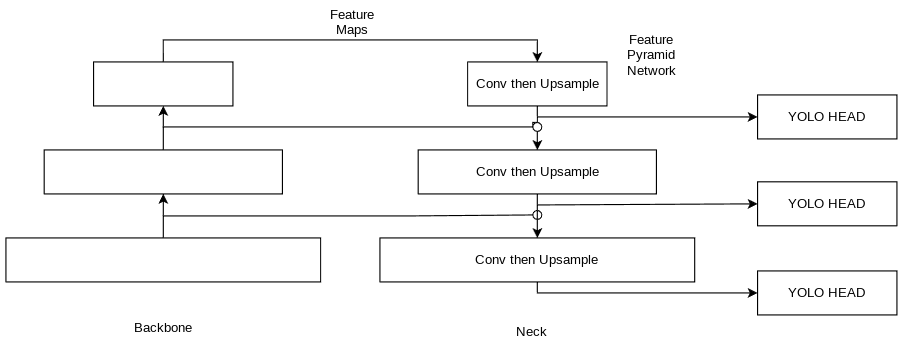
\includegraphics[scale=0.6]{figures/yolo-architecture-rough.png}
        \caption{Feature Pyramid Network in YOLOv3}
        \label{fig:yolofpn}
    \end{figure}

    The neck is the intermediate network between backbone and head.
    The main function of the neck is to enhance features extracted by the backbone.
    Specific implementation of neck for each YOLO architecture is different one to the other.
    Some neck implementation try to combine feature maps across different prediction scales of YOLO network.

    \textcite{yolov3} was the first to introduce YOLO prediction in multiple scale in YOLOv3.
    To enhance the feature maps with using information across scales, YOLOv3 fuses features 
    from multiple parts of the backbone before up sampling them as seen on Figure \ref{fig:yolofpn}. 
    This type of neck network is called Feature Pyramid Network (FPN). 
    A further improvement was made by \textcite{yolov4} with their YOLOv4 by introducing Path 
    Aggregation Network (PANet) for the neck. 
    With PANet, feature are fused back to higher scale by adding another FPN-like layer after the original FPN
    but with reverse direction.
    %The way it works is by taking feature maps, not only in the last output layer of the
    %backbone, but also in multiple parts of the backbone.
    %For example, YOLOv4 uses PANet to enhance and combine features across different scales
    %of prediction.
  
    %\emph{Neck} dari YOLO merupakan \emph{layer-layer} dimana \emph{head} YOLO mengambil fitur untuk dilakukan deteksi \emph{bounding box}.
    %Pada YOLOv3 \textcite{yolov3}, arsitektur \emph{neck} dibuat menyerupai \emph{Feature Pyramid Network} (FPN) seperti pada Gambar \ref{fig:yolofpn}. 
    %Pada versi-versi YOLO selanjutnya, bentuk \emph{neck} ini tidak banyak berubah dan pada dasarnya tetap mempertahankan bentuk \emph{pyramid}-nya.
  
    %Penaikkan tingkatan \emph{pyramid} dari FPN merupakan \emph{upsampling} dari \emph{feature map} yang dihasilkan \emph{backbone}.
    %Output tiap tingkatan pada FPN di \emph{neck} inilah yang diinputkan pada \emph{head} YOLO. 
    %Melakukan prediksi pada tingkatan \emph{upsampling} yang berbeda-beda dapat membuat \emph{neural network} mendapatkan lebih banyak informasi semantik dan informasi yang lebih detail sehingga dapat lebih akurat dalam mendeteksi objek besar maupun kecil.
 

  
    \subsubsection{The Head and The Anchors}
    \begin{figure}[H]
        \centering
        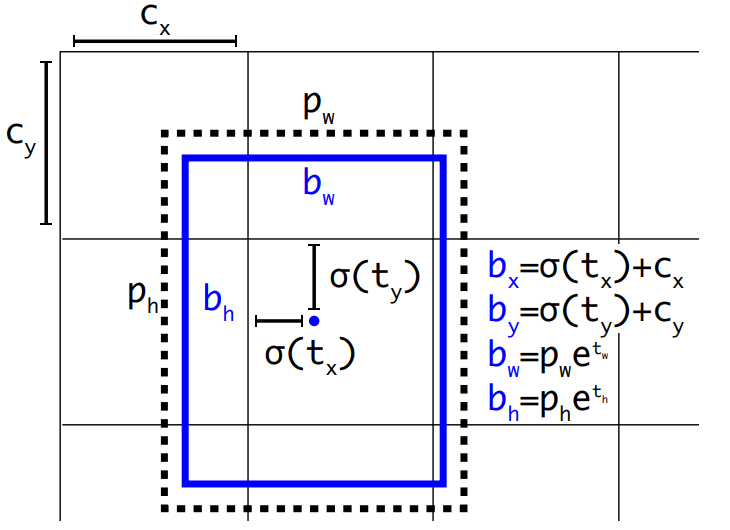
\includegraphics[width=0.5\textwidth]{figures/anchorbox.png}
        \caption{Head layer predict anchor box and its offsets from lattice of the feature grid \parencite{yolov3}}
        \label{fig:anchorbox}
    \end{figure}
    The head is where the object detection happens. Extracted and enhanced features of the image is fed to the head 
    in multiple different scales. For each scale, the head will predict a box for each $N \times N$
    lattice point on feature map's grid. In total, each layer will output a tensor with size
    $N_k \times N_k \times [A_k \times (4+1+C)]$ where $N_k$ is the size of feature map grid at the $k$-th scale,
    $A_k$ is the number of anchors for that scale, 4 is for the four offsets $[t_x, t_y, t_w, t_h]$ in figure 
    \ref{fig:anchorbox}, 1 is for the objectness score for the grid, and $C$ is for the number of classes it has
    to predict.
    
    Most of YOLO family architecture head utilizes anchor boxes to assist bounding box prediction.
    This technique is used in \textcites{yolov2}{yolov3}{yolov4}{scaledyolov4}{yolov5}{yolor}{yolov7}.
    Instead of directly predicting the size and position of the bounding box, YOLO head predicts 
    the offsets for each anchor boxes assigned to the head, then it utilizes the objectness score to pick
    which result  of these anchor boxes to be used.
    Using anchor boxes allows the neural network to converge more quickly because it provides
    a prior knowledge of the dataset before training.
    
    %The way it works is that, there will be a preset of detection boxes.
    %Arsitektur famili YOLO yang dipublikasikan setelah YOLOv2 terus menggunakan \emph{anchor box} untuk melakukan deteksi \parencites{yolov2}{yolov3}{yolov4}{scaledyolov4}{yolov5}{yolor}{yolov7}.
    %\emph{Anchor boxes} merupakan beberapa \emph{Bounding Box} yang telah terdefinisikan. 
    %Arsitektur YOLO akan memprediksi probabilitas \emph{anchor box} berada pada suatu koordinat latis beserta dengan \emph{offset anchor box} tersebut untuk menepatkan \emph{anchor box} pada objek yang dideteksi.
    %Penggunaan \emph{anchor box} ini dapat meningkatkan akurasi deteksi karena \emph{neural network} hanya perlu mencari titik tengah objek dan \emph{error} dimensi \emph{boudning box} dengan menggunakan \emph{offset} \parencite{yolov3}.
    %Hal ini lebih sederhana daripada mencari titik-titik \emph{bounding box} secara independen sehingga lebih mudah untuk dipelajari oleh \emph{neural network}.
  
    %Prediksi \emph{bounding boxes} terjadi di bagian \emph{head} dari arsitektur YOLO.
    %Bagian \emph{head} dari YOLO akan mengambil beberapa hasil \emph{upsampling} yang terjadi pada \emph{neck} YOLO, dan kemudian melakukan prediksi \emph{anchor boxes} dari hasil tersebut.
    %Hasil prediksi \emph{Head} YOLO pada suatu tingkatan \emph{upsampling} berupa tensor dengan ukuran $N\times N \times [A\times(4+1+C)]$ dengan $N$ sebagai dimensi hasil \emph{upsampling}-nya, $A$ sebagai jumlah \emph{anchor boxes} untuk \emph{scaling} tersebut, dan $C$ sebagai jumlah kelas prediksi.
    %Angka 4 merepresentasikan 4 \emph{offset} $b_x, b_y, b_w, b_h$ seperti pada Gambar \ref{fig:anchorbox} dan angka 1 merepresentasikan \emph{objectness score} dari prediksi \emph{bounding box}.

    \subsubsection{Loss Function}
    The goal of a YOLO architecture is to (1) predict if an object exist or not, (2) predict the bounding box of such object,
    and (3) predict the class of the object. These 3 loss functions that correspond to those objectives are called 
    objectness loss, box loss, and class loss respectively. To update the weights on training, the total loss is calculated as 
    the weighted sum of those 3 losses.
    %\begin{equation}
    %  L_{box} = \sum_{k=0}^{n}\sum_{i,j=0}^{N_k}\sum_{m=0}^{A_k} \mathbbm{1}_{k,i,j,m}^{obj} -IoU(gt(x), M(x)_{k,i,j,m})
    %\end{equation}
    In original YOLO, the loss functions were defined like the following.

    For localization loss, it is described by equation \ref{eq:yolo-box-loss}.
    \begin{equation}
      L_{box} = \sum_{i=0}^{S^2} \sum_{j=0}^B \mathbbm{1}_{ij}^{obj} \left[(x_i - \hat{x}_i)^2 + (y_i - \hat{y}_i)^2 + (\sqrt{w_i}-\sqrt{\hat{w}_i})^2 + (\sqrt{h_i}-\sqrt{\hat{h}_i})^2\right] \\
      \label{eq:yolo-box-loss}
    \end{equation}
    \begin{align*}
    \text{Where}~S^2  &= \text{the total number of grid cells in the output,}\\
    B &= \text{ the total number of anchor box per grid cells,}\\
    \mathbbm{1}_{ij}^{obj} &= \begin{cases}
                                1, & \text{if object present in grid}\\
                                0, & \text{otherwise,}
                              \end{cases} 
                              \\
    (x_i, y_i) &= \text{the predicted coordinates of the center of object i}\\
    (\hat{x}_i, \hat{y}_i) &= \text{the ground truth coordinates of the center of object}\\
    (w_i, h_i) &= \text{the predicted width and height of object i}\\
    (\hat{w}_i, \hat{h}_i) &= \text{the ground truth width and height of object}
      %\text{the indicator variable that has value 1 if object is present in the grid and 0 otherwise.}
    \end{align*}
    %$\mathbbm{1}_{ij}^{obj}$ is the indicator variable that has value 1 if object is present in the grid and 0 otherwise.
    %$(x_i, y_i)$ and $(\hat{x}_i, \hat{y}_i)$ are the predicted and ground truth coordinates of the center of object $i$.
    %$(w_i, h_i)$ and $(\hat{w}_i, \hat{h}_i)$ are the predicted and ground truth widths and heights of object $i$.
    For objectness loss, described by equation \ref{eq:yolo-obj-loss}
    \begin{equation}
      L_{obj} = \sum_{i=0}^{S^2} \sum_{j=0}^B \mathbbm{1}_{ij}^{obj}(C_i - \hat{C}_i)^2  + \alpha \mathbbm{1}_{ij}^{noobj}(C_i - \hat{C}_i)^2
      \label{eq:yolo-obj-loss}
    \end{equation}
    \begin{align*}
    Where~\mathbbm{1}_i^{\text{noobj}} &=\begin{cases} 
                                          1, & \text{if object assigned to anchor j}\\
                                          0, & \text{otherwise} 
                                         \end{cases}\\
          (C_i,\hat{C}_i) &= \text{predicted and ground truth confidence score for objectness of anchor}
    \end{align*}
    %$(C_i, \hat{C}_i)$ are the predicted and ground truth confidence scores for objectness of anchor $i$,
    And for class loss, described by \ref{eq:yolo-class-loss}
    \begin{equation}
      L_{class} = \sum_{i=0}^{S^2} \mathbbm{1}_{ij} \sum_{c \in classes} (p_i(c) - \hat{p}_i(c))^2
      \label{eq:yolo-class-loss}
    \end{equation}
    Where $(p_i(c), \hat{p}_i(c))$ are the predicted and ground truth class probabilities for class $c$ for object $i$.

    The three losses combined to the final loss function in equation \ref{eq:yolo-loss}
    \begin{equation}
      L = \lambda_{box}L_{box} + \lambda_{obj}L_{obj} + \lambda_{class}L_{class}
      \label{eq:yolo-loss}
    \end{equation}
    \begin{align*}
      Where~\lambda_{box} &= \text{the weight for localization,}\\
      \lambda_{obj} &= \text{weight for objectness}\\
      \lambda_{class} &= \text{weight for class}
    \end{align*}
    These 3 $\lambda$-s can be tuned to optimize the performance of a YOLO network.

    %\begin{equation}
    %  L_{box} = \sum_{i=0}^{S^2}\sum_{j=0}^B   \mathbbm{1}_{ij}^{obj} (x_i-\hat{x}_i)^2 + (y_i-\hat{y}_i)^2 + (\sqrt{w_i}-\sqrt{\hat{w}_i})^2 + (\sqrt{h_i}-\sqrt{\hat{h}_i})^2 
    %\end{equation}
      %L_{box} = \sum_{k=0}^{n}\sum_{i,j=0}^{N_k}\sum_{m=0}^{A_k} \mathbbm{1}_{k,i,j,m}^{obj} -IoU(gt(x), M(x)_{k,i,j,m})

    %\begin{equation}
    %  L_{box} = 1
    %\end{equation}

  
      
  \subsection{YOLOv7}
  As said in section \ref{section:background}, YOLOv7 is the state-of-the-art real-time object detector.
  It was made by the authors of YOLOv4, and by the time it was published (july 2022), it surpassed all 
  known real-time object detectors both in speed and accuracy. To achieve this, YOLOv7 implemented some new
  changes and addition to the neural network. 
  \subsubsection{Backbone}

%  \vspace{-2ex}
  %\begin{figure}[H]
  %    \centering
  %    \subfigure[ELAN block]{
  %    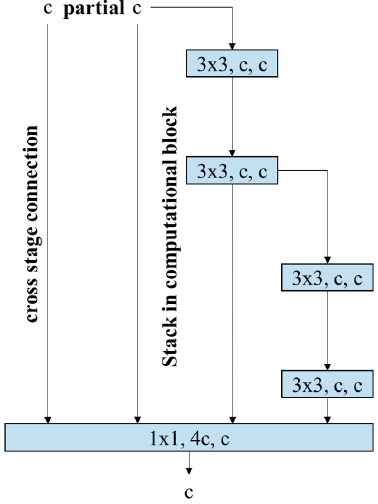
\includegraphics[width=0.2\textwidth]{figures/elan-block.png}
  %    \label{fig:elan-block}
  %    }
  %    \subfigure[FIGTOPCAP][First two ELAN blocks in YOLOv7]{
  %    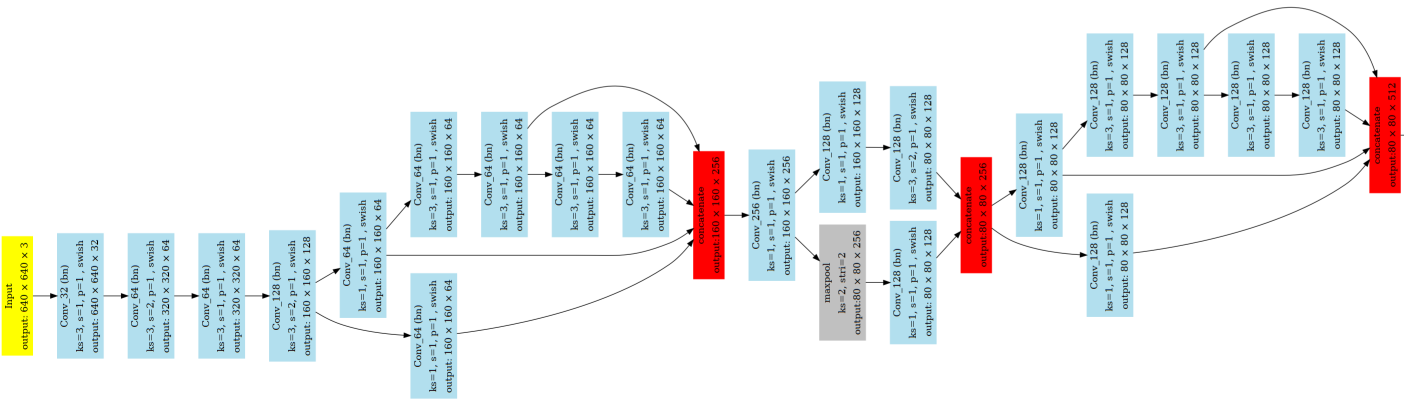
\includegraphics[width=0.75\textwidth]{figures/yolo-elan-blocks.png}
  %    \label{fig:elan-yolo}
  %    }
  %    \caption{ELAN in YOLOv7}
  %    \label{fig:elan}
  %\end{figure}
  \begin{figure}[H]
    \centering
    \begin{subfigure}[c][][c]{.4\textwidth}
        %%%\vspace{0pt}
        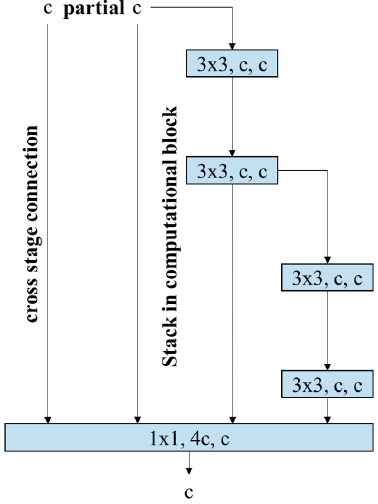
\includegraphics[width=1\linewidth]{figures/elan-block.png}
        \caption{ELAN block}
        \label{fig:elan-block}
    \end{subfigure}

    \begin{subfigure}[c][][c]{.9\textwidth}
        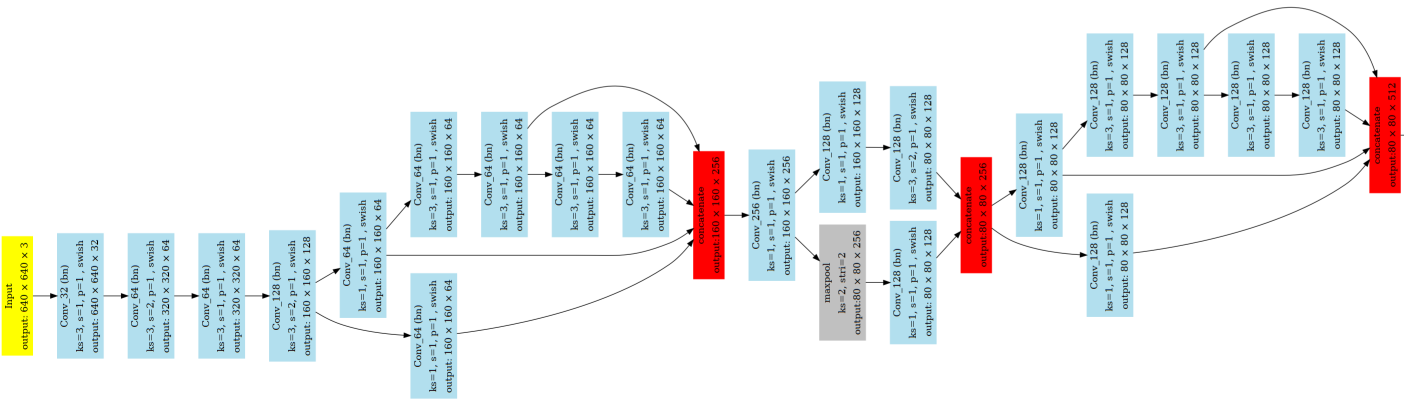
\includegraphics[width=1\linewidth]{figures/yolo-elan-blocks.png}
        \caption{First two ELAN blocks in YOLOv7}
        \label{fig:elan-yolo}
    \end{subfigure}

    \caption{ELAN in YOLOv7}
    \label{fig:elan}
  \end{figure}

  %remove this negative vspace if buku TA kurang panjang

  YOLOv7 implemented Efficient Layer Aggregation Network (ELAN) and Extended-ELAN (E-ELAN) as the backbone. 
  ELAN is a convolutional neural network that was designed to extract features efficiently 
  by controlling the shortest longest gradient path in the network \parencite{elan}.
  This choice of backbone allows YOLOv7 to perform prediction more accurately despite having fewer number of parameters. 
  Figure \ref{fig:elan-yolo} shows how ELAN block in Figure \ref{fig:elan-block} implemented in YOLOv7.

  \subsubsection{Label Assignment Strategy and Auxilary Head}
  \begin{figure}[H]
      \centering

      \begin{subfigure}[][][t]{0.5\textwidth}
        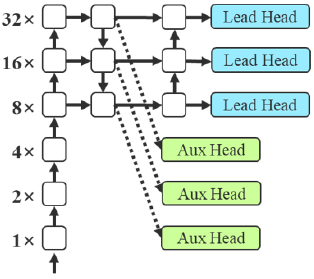
\includegraphics[width=1\linewidth]{figures/auxilary-head.png}
        \caption{Auxliary heads attachment in YOLOv7}
        \label{fig:aux-head}
      \end{subfigure}

      \begin{subfigure}[][][t]{0.4\textwidth}
        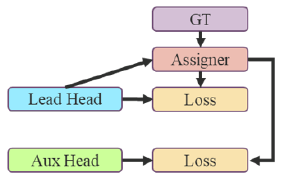
\includegraphics[width=1\linewidth]{figures/lead-head-assigner.png}
        \caption{Lead guided label assignment}
        \label{fig:lead-head}
      \end{subfigure}\hfill
      \begin{subfigure}[][][t]{0.4\textwidth}
        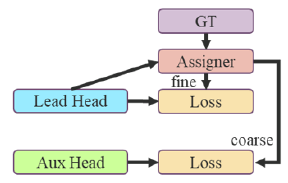
\includegraphics[width=1\linewidth]{figures/coarse-to-fine.png}
        \caption{Coarse-to-fine lead guided label assignment}
        \label{fig:coarse-to-fine}
      \end{subfigure}

      \caption{YOLOv7 Label Assignment Strategy with Auxilary Heads}
      \label{fig:labelassigner}
  \end{figure}
  SimOTA, first introduced in YOLOX, is an algorithm to approximate Optimal Transport Assignment (OTA)
  in a faster way. \textcite{yolox} introduced SimOTA in YOLOX because OTA was deemed too slow to compute
  as it was increasing the training time by 25\%. YOLOv7 also implemented SimOTA for its dynamic label assigner.

  YOLOv7 deep supervised its training process by attaching auxilary heads to its neural network
  as seen on Figure \ref{fig:aux-head}.
  These auxilary heads is only used on training, on inference, they are removed from the neural network
  to improve latency, only the lead head is kept. There is a problem however with assigning labels
  to the auxilary and lead heads. Most object detection networks that utilizes auxilary heads have 2
  independent label assigners, one for auxilary heads and one for lead heads. YOLOv7 done things differently.


  YOLOv7 proposed 2 way of assigning labels to auxilary and lead heads. Lead head guided label assignment (Figure \ref{fig:lead-head}) and
  coarse-to-fine lead head guided assignment (Figure \ref{fig:coarse-to-fine}). For lead head guided label assignment, the assigner gives a copy
  of lead heads' label assignment to the auxilary heads. For coarse-to-fine lead head guided assignment, the 
  assigner works like lead head guided assigner but gives coarse label assignment to auxilary head. Coarse label
  assignment is done by relaxing the positive sample constraints of the assigner. \textcite{yolov7} find that coarse-to-fine
  label assignment produces the greatest AP scores.
  
  Due to the relaxed constraints, coarse label assignment to auxilary heads assigns more positive labels the auxilary heads' grids. 
  This way, the network will learn more to recall.
  On inference, this recall ability would be filtered by the lead head to produce accurate prediction.
  \subsubsection{Reparameterization}
  YOLOv7 utilized RepConv and YOLOR implicit layers in its network.
  These 2 layers can be reparameterized after training to simplify the neural network, thereby reducing
  latency and memory usage but not hurting inference performance.
    %YOLOv7 merupakan pendeteksi objek \emph{real time} dengan skor akurasi tertinggi pada dataset COCO di tahun 2022.
    %Pada YOLOv7, dilakukan beberapa perubahan untuk meningkatkan akurasi dan kecepatan deteksinya.
    %Perubahan-perubahan tersebut dilakukan pada arsitekturnya dan pada \emph{bag-of-freebies}-nya.
  
    %Perubahan arsitektur dilakukan pada \emph{backbone}. YOLOv7 menggunakan \emph{Extended Efficient Layer Aggregation Network} (E-ELAN) sebagai \emph{backbone}, berbeda dengan leluhurnya YOLOv4 yang menggunakan CSP-Darknet.
    %E-ELAN merupakan arsitektur \emph{neural network} yang efisien karena E-ELAN didesain dengan mengontrol \emph{gradient path} terpanjang yang terpendek.
    %Karena efisiensinya, arsitektur E-ELAN ini dapat meningkatkan kecepatan deteksi dan akurasi. \parencite{yolov7}
  
    %\emph{Bag-of-freebies} merupakan kumpulan metode peningkatan akurasi yang tidak meningkatkan \emph{cost inferrence} \parencite{yolov4}. 
    %Pada YOLOv7, ditambahkan beberapa \emph{bag-of-freebies} yang dapat dilatih seperti \emph{re-parameterized convolution} dan \emph{extra auxilary head} di tengah-tengah \emph{neural network}.
    %Selain kedua itu, YOLOv7 juga menambahkan \emph{trainable bag-of-freebies} dari YOLOR seperti EMA, \emph{Implicit Knowledge}, dan \emph{conv-bn topology Batch Normalization} \parencite{yolov7}.
    %Introducing YOLOv7, a state-of-the-art deep learning based real-time object detector \parencite{yolov7}.
    %At the time of the proposal for this research was made (November 2022),
    %YOLOv7 outperform both in speed and accuracy of all known real-time object detectors 
    %with inference speed in the range of 5-160 FPS. It also has the highest accuracy (56.8\% AP) among
    %object detectors with inference speed greater than 30 FPS on a V100 GPU. The capabilities of this cutting-edge architecture
    %makes it well-suited for AAV computer vision system. However, all the performance metrics of YOLOv7
    %mentioned before are obtained by training the model using COCO 2017 dataset. A dataset which 
    %consist of general objects that people see in their daily life. COCO dataset is going to have
    %very distinct distribution compared to airborne objects. As such, there would be a need for
    %some modification to YOLOv7 so that it could detect airborne objects well.


  \subsection{Anchor Recalculation}
  \label{section:anchor_recalc_study}
  Anchor recalculation is a common method of introducing prior distribution of the dataset to an anchor-based object
  detection networks. Most of the time, anchors provided by pretrained YOLO weights are optimized for the common metrics
  dataset such as COCO2017 or VOC2012. Thus, recalculating anchor can help the neural network learn faster.

  There are multiple ways of recalculating anchors. Some of them can be performed before training or during training.
  Most of pre-training anchor recalculation method involves with clustering the anchors to the dataset. This is done by
  using clustering algorithm such as K-means, Gaussian Mixture, and many others. Recalculating anchor on training is 
  a little more complex to do as it will involve some loss function or architectural change on the object detection neural network.
  \textcite{anchoropt} for example add additional layer on detection part of object detectors that is connected to anchor modifiers such that
  the anchors will also be updated during training. \textcite{yolor} mentioned that the implicit multiplication layer of their network
  can be purposed for anchor refinement.

  %\emph{Anchor box} dari model-model \emph{pre-trained} YOLO pada umumnya mengoptimisasi \emph{anchor box} modelnya pada dataset COCO.
  %Ukuran \emph{anchor box} yang akan digunakan pada model YOLO dapat dikonfigurasikan agar lebih sesuai dengan dataset yang akan digunakan untuk melatih model YOLO.
  %Penyesuaian ini dapat meningkatkan IoU(\emph{Intersection Over Union}) prediksi model dengan \emph{ground truth} sehingga meningkatkan akurasi.

  %Penyesuaian anchor box dapat dilakukan pada saat sebelum training atau pada saat training.
  %Penyesuaian anchor box sebelum training dapat dilakukan dengan cara mengkonfigurasi secara manual tiap ukuran \emph{anchor box} atau dengan menggunakan algoritma \emph{clustering}.
  %Penggunaan algoritma \emph{clustering} akan lebih baik karena setiap ukuran \emph{anchor box}-nya disesuaikan dengan pengelompokan-pengelompokan ukuran \emph{bounding box} natural yang terdapat pada dataset.
  %Untuk penyesuaian saat training, dapat digunakan algoritma dari \textcite{anchoropt}.
  %Algoritma ini akan mengoptimisasi ukuran-ukuran anchor bukan hanya berdasarkan dataset, namun berdasarkan kemampuan dari neural network pendeteksi objeknya.
  %Untuk melakukan hal tersebut, algoritma ini akan memanfaatkan back propagation localization loss untuk rekalkulasi anchor.

  \subsection{Mosaic Augmentation}
  \label{section:mosaic_study}
  \begin{figure}[H]
    \centering
    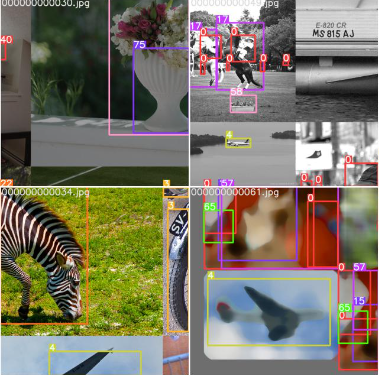
\includegraphics[width=0.5\textwidth]{figures/mosaic-aug.png}
    \caption{Four example of mosaic augmentation \parencite{yolov5}}
    \label{fig:mosaic}
  \end{figure}
  Mosaic augmentation was introduced in Ultralytics' implementation of YOLOv3 \parencite{mosaic_aug}.
  This augmentation technique will randomly pick 4 images of the dataset, and tile them randomly into one image like in \ref{fig:mosaic}.
  It's called mosaic due to how the result of the augmented image have mosaic-like appereance.
  \textcites{cspnet}{yolov4}{yolov5} reported increase in accuracy after applying mosaic augmentation.
  %Augmentasi mosaik merupakan teknik augmentasi yang baru dikenalkan pada YOLOv4.
  %Teknik augmentasi ini akan memilih 4 gambar dari dataset, memotong gambar-gambar tersebut dan menggabungkannya secara acak pada satu gambar seperti pada Gambar \ref{fig:mosaic}.
  %Hasil dari penggabungan itu membuat gambar terlihat seperti mosaik.
  %Teknik augmentasi ini mampu meningkatkan akurasi model \parencite{yolov4}.


\section{Related Works}
\label{section:relatedwork}

  \subsection{YOLO-Z}
  \begin{figure}[H]
    \centering
    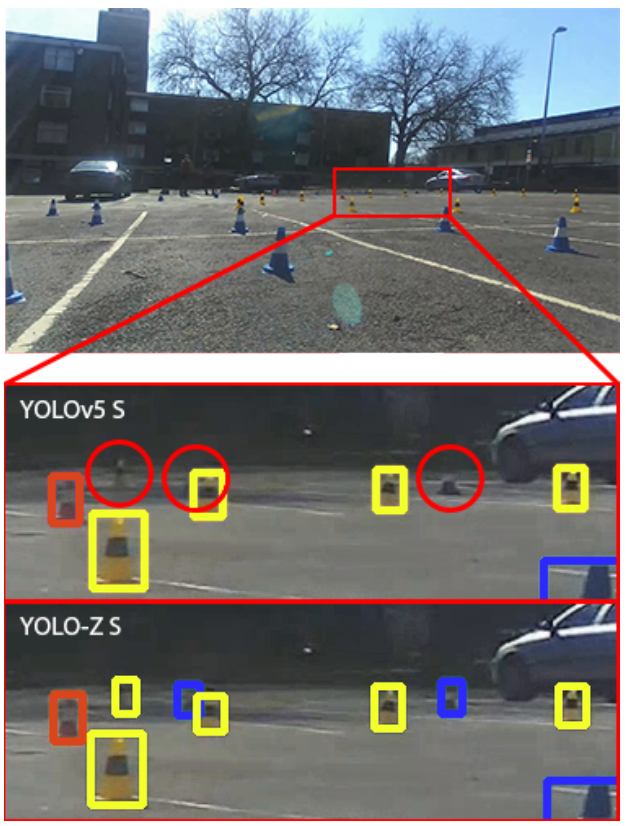
\includegraphics[width=.4\textwidth]{figures/yoloz-result.png}
    \caption{Small objects in the image. Comparison of YOLOZ-S and YOLOv5-S. YOLOv5-S was not able to detect the circled objects.}
    \label{fig:yolozcone}
  \end{figure}
  YOLO-Z is a derivative architecture of YOLOv5r5.0.
  This variant of YOLO modified the backbone, neck, and number of anchors of the original YOLOv5 to 
  enhance its capability of detecting small objects \parencite{yoloz}.
  These changes are backbone change from YOLOv5r5.0 to a downscaled DenseNet,
  neck change from FPN to biFPN on some YOLO-Z scales, and increasing the number of anchors used at each scale.

  YOLO-Z was aimed to be used in autonomous racing car. In this high speed environment, early detection
  of obstacle is crucial to plan for action. For that reason, the autonomous racing car must detect the cone-shaped obstacles
  that are far away from it. Since objects that are far away appear small on image captured by camera, YOLOv7 was designed with
  purpose of small object detection.
  %YOLO-Z merupakan arsitektur famili YOLO yang modifikasi dari YOLOv5 \parencite{yoloz}.
  %Modifikasi-modifikasi yang dilakukan meliputi pergantian \emph{backbone}, \emph{neck}, dan jumlah \emph{anchor}
  %\emph{Backbone} dari YOLOv5r5.0 menjadi DenseNet yang di-\emph{downscale}.
  %\emph{Neck} dari YOLO-Z juga diganti dari PanNet menjadi FPN dan biFPN tergatung pada \emph{scale} YOLO-Z yang digunakan.

  %Modifikasi pada YOLO-Z didesain untuk mendeteksi objek kecil untuk tujuan melakukan deteksi \emph{cone} yang nampak jauh pada lintasan \emph{autonomous racing} secara \emph{real time} (lihat Gambar \ref{fig:yolozcone}).
  %Modifikasi-modifikasi dibuktikan dapat meningkatkan kemampuan pendeteksian objek kecil \parencite{yoloz}.
  %Oleh karena itu, untuk meningkatkan kemampuan mendeteksi objek kecil YOLOv7, beberapa modifikasi yang dilakukan YOLO-Z pada YOLOv5 dapat diaplikasikan.

  \subsection{exYOLO}
  exYOLO is a modification of YOLOv3 \parencite{exyolo}.
  exYOLO added a Receptive Field Block before feature-fusion in the neck to one of the feature scale.
  This change made exYOLO produce a higher mAP score on VOC2007 compared to its baseline YOLOv3.
    %exYOLO merupakan hasil modifikasi arsitektur YOLOv3 \parencite{exyolo}.
    %Pada exYOLO, dilakukan modifikasi \emph{neck} dengan menambahkan suatu \emph{Receptive Field Block} sebelum penggabungan \emph{feature map} yang akan diupsampling.
    %Modifikasi-modifikasi ini membuat exYOLO memiliki skor mAP yang lebih tinggi daripada YOLOv3 pada dataset PASCAL VOC 2007.

  \subsection{YOLOv4-tiny with added head}%Implementasi YOLOv4-tiny pada \emph{Autonomous Surface Vehicle}}
  \begin{figure}[H]
    \hfill%
    \begin{subfigure}[c][][c]{.45\textwidth}
        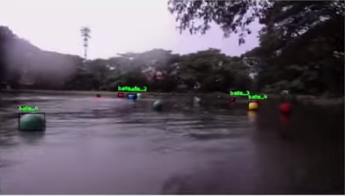
\includegraphics[width=1\linewidth]{figures/yolov4barun-regular.png}
        \caption{Regular YOLOv4-tiny prediction}
        \label{fig:barun-yolov4}
    \end{subfigure}\hfill  
    \begin{subfigure}[c][][c]{.45\textwidth}
        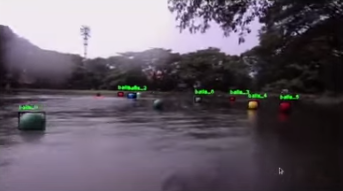
\includegraphics[width=1\linewidth]{figures/yolov4barun-addhead.png}
        \caption{YOLOv4-tiny with added head prediction}
        \label{fig:barun-yolov4-3l}
    \end{subfigure}\hfill%
    \caption{Comparison of regular YOLOv4-tiny and YOLOv4-tiny with added head on \textcite{barunastra} ASV}
    \label{fig:barun}
  \end{figure}

  \textcite{barunastra} used YOLOv4-tiny as their Autonomous Surface Vehicle (ASV) object detector due to the computational
  device constraint.
  To detect objects that were atleast 30 meters away from the ASV, they applied a modification of YOLOv4-tiny, which was YOLOv4-tiny
  but with additional head layer. The original YOLOv4-tiny only had 2 head layers, thus was only predicting in 2 scales.
  An addition of head layer allows it to predict in 3 scales. Using this modification, the network was able to detect small object
  better and raised the overall mAP score by 4\% without significantly reducing latency.

  %\textcite{barunastra} menggunakan model modifikasi YOLOv4-tiny pada \emph{Autonomous Surface Vehicle}(ASV) mereka.
  %YOLOv4-tiny sebenarnya hanya menggunakan 2 layer head, namun yang diimplementasikan pada ASV adalah model YOLOv4-tiny
  %yang ditambahkan 1 layer head lagi sehingga menggunakan total sebanyak 3 layer head. Perubahan ini memberikan peningkatan
  %pada skor mAP dan memberikan kemampuan modelnya untuk mendeteksi objek yang lebih jauh.